\section{Durchführung}
\label{sec:Durchführung}

%Was wurde gemessen bzw. welche Größen wurden variiert?

\subsection{Abstimmung der Resonanzfrequenz}
\label{sec:resonanz}

\begin{figure}
    \centering
    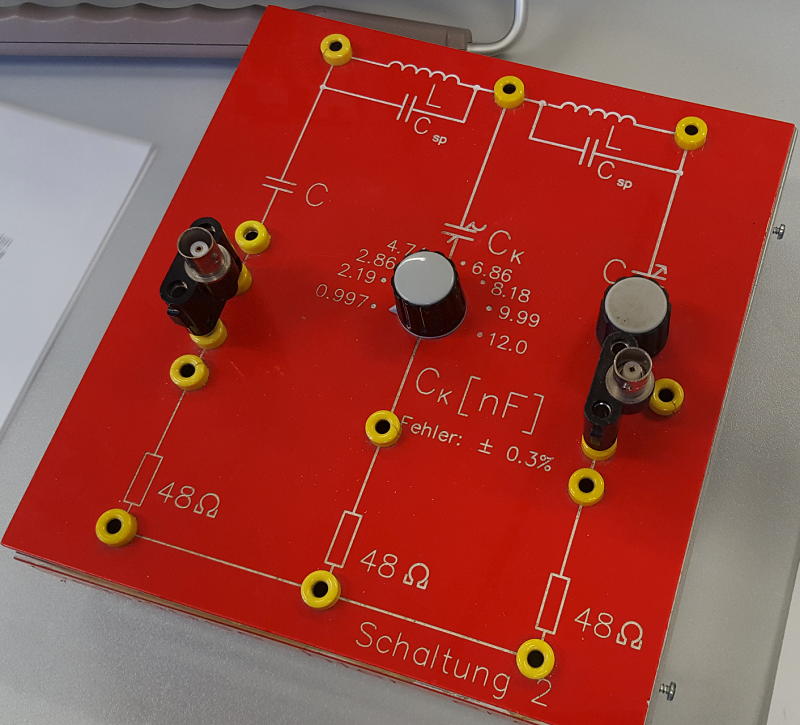
\includegraphics[width=\textwidth/2]{images/foto_01.png}
    \caption{Foto des genutzten Schaltkastens}
    \label{fig:foto_01}
\end{figure}
Gegeben ist der Schaltkasten wie in \autoref{fig:foto_01} zu sehen ist.
Da beide Schwingkreise die gleiche Resonanzfrequenz haben sollen, muss diese für den linken Schaltkreis zunächst ermittelt werden, um dann den rechten Schaltkreis daran anzupassen.

\begin{figure}
    \centering
    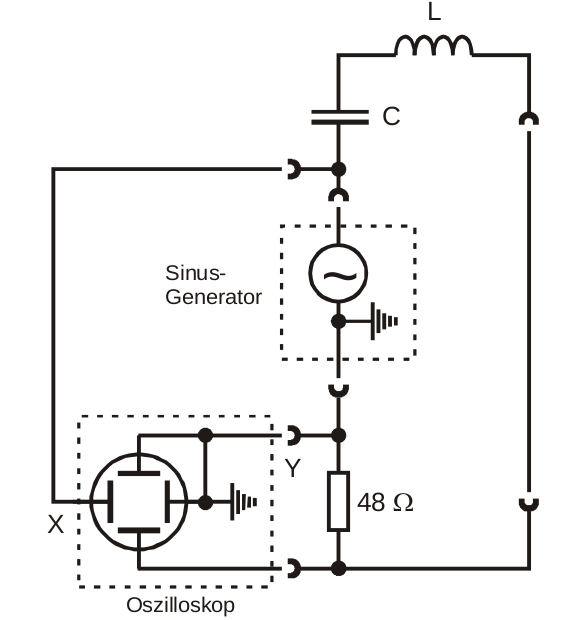
\includegraphics[width=\textwidth/3]{images/schaltung_3.png}
    \caption{Schaltung zur Kalibrierung\cite{V355}}
    \label{fig:schaltung_3}
\end{figure}
Hierzu wird am linken Schwingkreis ein Oszilloskop und ein Sinusgenerator wie in \autoref{fig:schaltung_3} angeschlossen. 
Um nun die Resonanzfrequenz zu messen wird am Sinusgenerator die Frequenz solange verstellt bis die am Oszilloskop abgebildete Lissajous-Figur eine Ellipse ist, welche symmetrisch zur x- und y-Achse ist. Somit ist die Phasenverschiebung zwischen Generatorspannung und Schwingkreisspannung $\pi/2$. 
Nun wird die eingestellte Frequenz als Resonanzfrequenz notiert.
Dann muss die gleiche Schaltung mit gleicher Generatorfrequenz für den rechten Schwingkreis aufgebaut werden.
Der dort eingebaute Kondensator wird nun so eingestellt dass auch hier die Lissajous-Figur eine Gerade ist. Nun sind die Schwingkreise nahezu identisch und die eigentliche Messung kann beginnen.

\subsection{Messung des Schwebungs-Schwingungs-Verhältnisses}
\label{sec:schwebung}

\begin{figure}
    \centering
    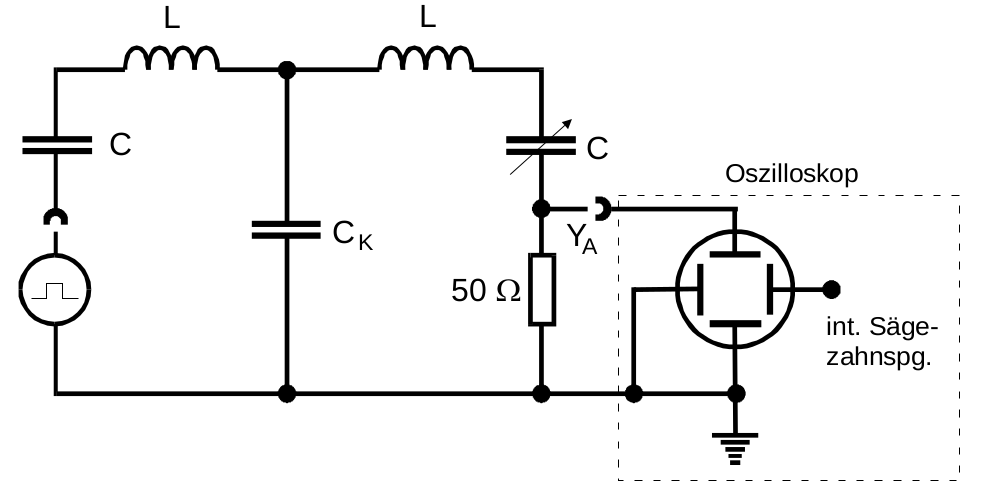
\includegraphics[width=\textwidth/2]{images/schaltung_4.png}
    \caption{Schaltung zur Untersuchung der gekoppelten Schwingkreise\cite{V355}}
    \label{fig:schaltung_4}
\end{figure}

Nun wird die Schaltung aus \autoref{fig:schaltung_4} aufgebaut.
Am Generator wird die Frequenz $\SI{626}{\hertz}$ eingestellt, da mit dieser die Schwebung gut am Oszilloskop zu sehen ist. Die Anzahl der Maxima und Extrema innerhalb eines Nulldurchgangs der Schwebung werden abgezählt und notiert. 
Dies wird für verschiedene Kopplungskapazitäten wiederholt.

\begin{figure}
    \centering
    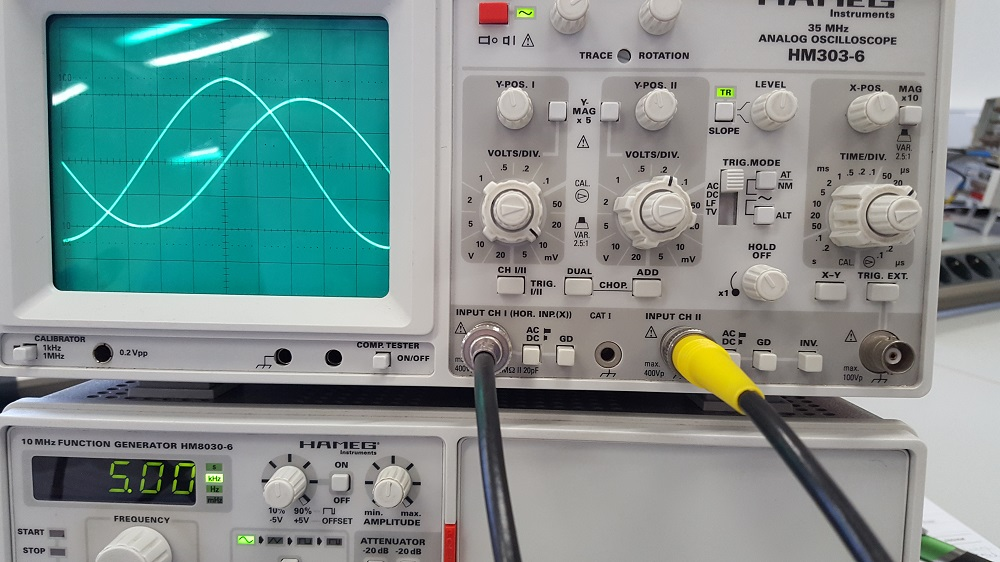
\includegraphics[width=\textwidth/2]{images/foto_03.jpg}
    \caption{Foto der Schwebung für $C_k = \SI{6.680}{\nano\farad}$}
    \label{fig:foto_03}
\end{figure}

\subsection{Messung der Fundamentalfrequenzen}
\label{sec:frequenzen}

Damit die Fundamentalfrquenzen der gekoppelten Schwingkreise gemessen werden können, wird nun wieder die Schaltung aus \autoref{fig:schaltung_4} verwendet.
Allerdings wird statt einer Rechteckschwingung eine Sinusschwingung verwendet und es wird auch die Generatorspannung auf das Oszilloskop gegeben.
Für verschiedene Kopplungskapazitäten werden am Generator die Frequenzen gesucht, welche die Lissajous-Figur zu einer Gerade werden lassen. 
Falls diese Gerade eine positive Steigung hat, wurde gleichschwingende Fundamentalschwingung gefunden und die Frequenz wird als $\nu _+$ notiert.
Eine Gerade negativer Steigung wird angezeigt, wenn die gegenphasige Fundamentalschwingung gefunden wurde. Hier wird die Frequenz als $\nu _-$ notiert.
\begin{figure}
    \centering
    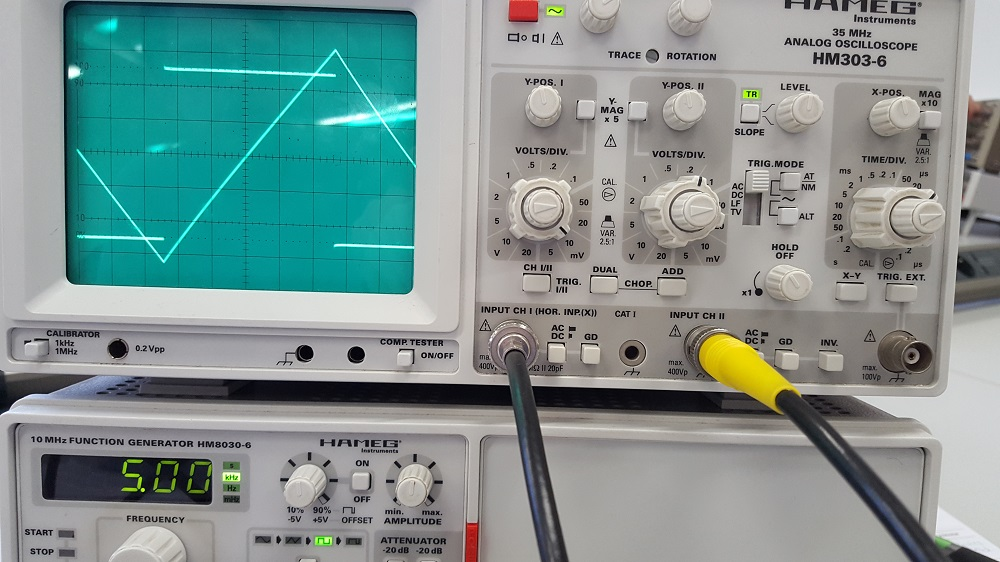
\includegraphics[width=\textwidth/2]{images/foto_05.jpg}
    \caption{Foto der Lissajous-Figur für $C_k = \SI{6.860}{\nano\farad}$ bei der gegenphasigen Fundamentalschwingung}
    \label{fig:foto_05}
\end{figure}

\subsection{Messung der Spannungsamplitude im Falle der Fundamentalschwingungen}
\label{sec:amplituden}

Da im Folgenden die Skalierung des im Oszilloskop angezeigten Bildes wichtig wird, muss nun dieser mithilfe einer breits bekannten Spannungsamplitude (z.B. des Generators) kalibriert werden.

Mit gleichem Schaltaufbau wie in \autoref{fig:schaltung_4} wird nun die Amplitude der Spannung der beiden Fundamentalschwingungen am rechten Widerstand gemessen. Außerdem wird auch die Spannung am mittleren Widerstand (siehe \autoref{fig:foto_01}) gemessen, wobei der rechte Widerstand überbrückt wird.
Dies wird wieder für verschiedene Kopplungskapazitäten durchgeführt.

Zur Referenz wird nun auch noch die Amplitude der Generatorspannung in den Fällen der Fundamentalschwingungen und einer Nicht-Fundamentalschwingung gemessen.

\begin{figure}
    \centering
    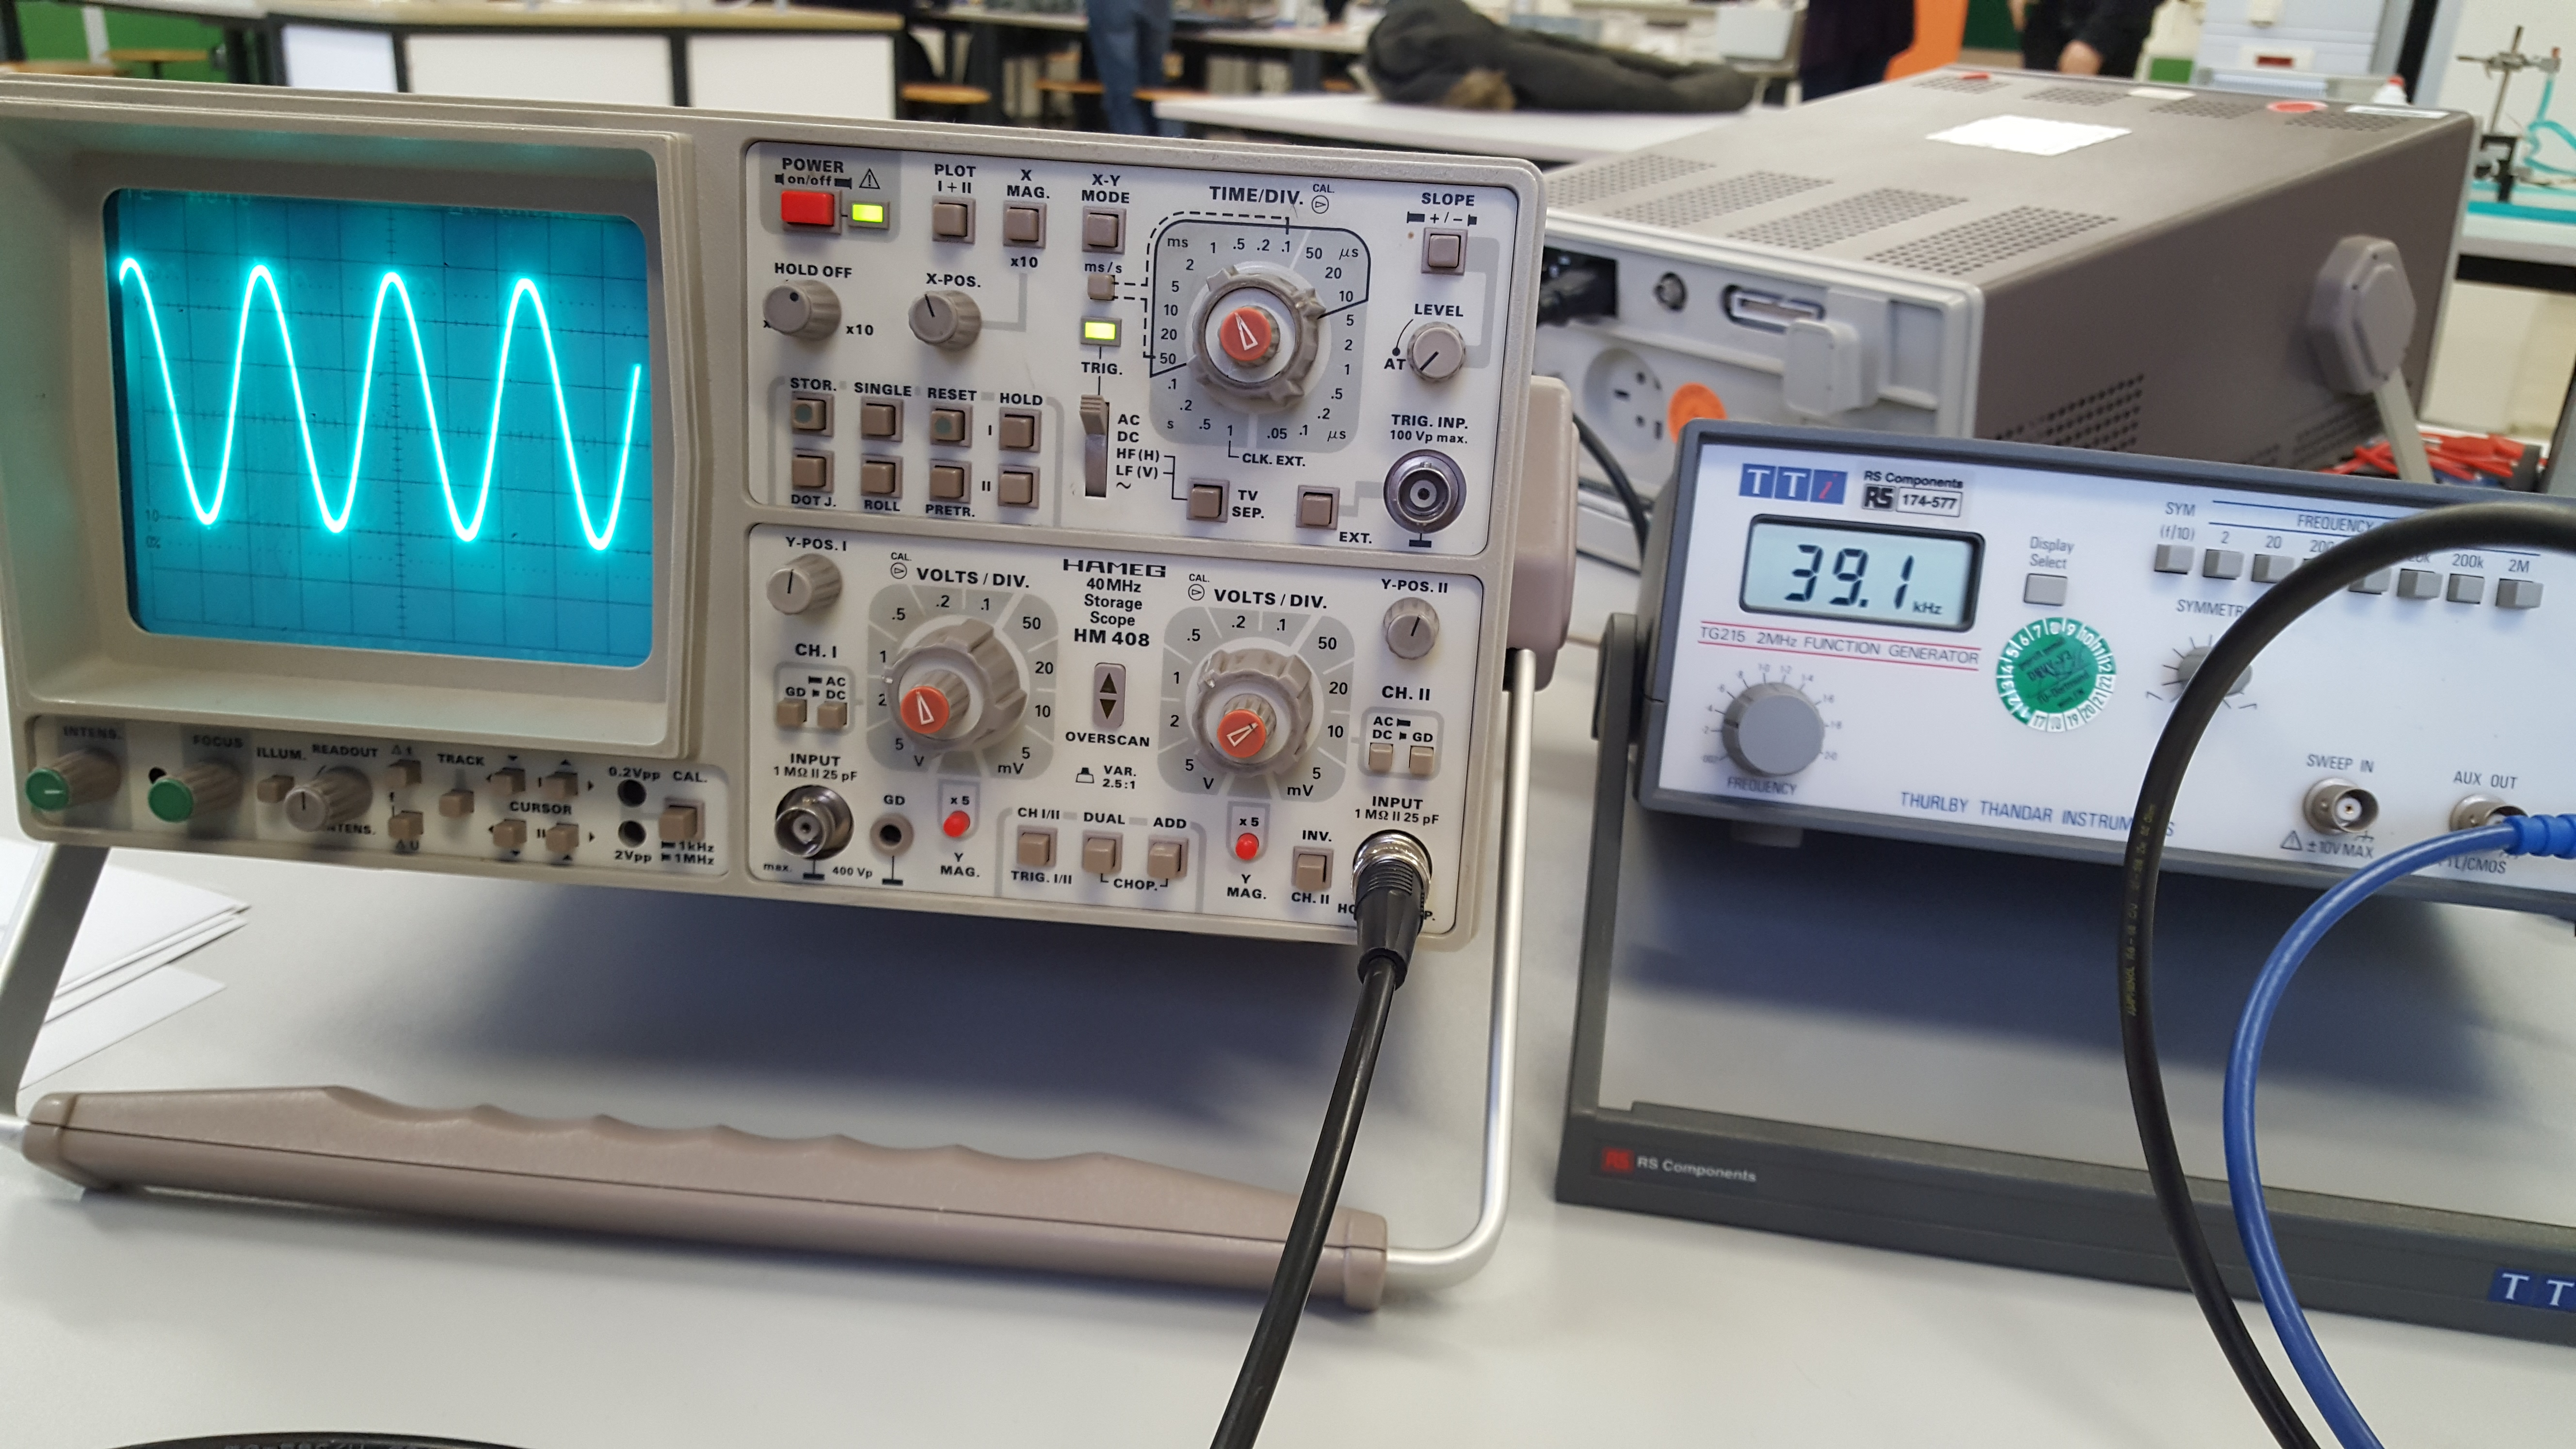
\includegraphics[width=\textwidth/2]{images/foto_10.jpg}
    \caption{Foto der abgelesenen Spannungsamplitude für $C_k = \SI{8.180}{\nano\farad}$ und der zugehörigen Resonanzfrequenz $v_+ = \SI{39.1}{\kilo\hertz}$}
    \label{fig:foto_10}
\end{figure}